\section{概念设计}\label{sec:concept}
\subsection{E-R图}
根据上述的需求分析,在本次设计的数据库中,包含以下实体集:
\begin{itemize}
  \item \textit{bike}:拥有属性(\textit{\underline{bike\_ID},production\_date,coordinate,valid});
  \item \textit{collection}:拥有属性(\textit{\underline{collection\_ID},time});
  \item \textit{reallocation}:拥有属性(\textit{\dotuline{reallocation\_ID},start\_time,start\_coordinate,end\_time,end\_coordinate});
  \item \textit{release}:拥有属性(\textit{\underline{release\_ID},coordinate,time});
  \item \textit{trace}:拥有属性(\textit{\underline{trace\_ID},start\_time,start\_coordinate,end\_time,end\_coordinate});
  \item \textit{type}:拥有属性(\textit{\underline{type\_ID},name,release\_date});
  \item \textit{user}:拥有属性(\textit{\underline{user\_ID}});
  \item \textit{warehouse}:拥有属性(\textit{\underline{warehouse\_ID},capacity,load,coordinate}),
\end{itemize}
并且包含以下关系集:
\begin{itemize}
  \item \textit{bike\_collection}:将单车回收工单、单车和仓库关联在一起;
  \item \textit{bike\_reallocation}:将单车调度工单和单车关联在一起;
  \item \textit{bike\_release}:将单车投放工单、单车和仓库关联在一起;
  \item \textit{bike\_type}:将单车和单车型号关联在一起;
  \item \textit{stored\_in}:将单车和仓库关联在一起;
  \item \textit{usage}:将单车、单车轨迹和用户关联在一起;
  \item \textit{user\_feedback}:将单车和用户关联在一起,
\end{itemize}

图\ref{fig:E-R diagram}是由以上实体集和关系集组合形成的E-R图。

下面将对各个实体集和关系集展开介绍。
\begin{figure}[htbp]
  \centering
  \includegraphics{figures/E-R_diagram.pdf}
  \caption{E-R图}
  \label{fig:E-R diagram}
\end{figure}
\subsection{实体集设计}
\paragraph{\textit{bike}}
该实体集的拓展是在现实中公司所拥有的单车。

该实体集有以下属性:
\begin{itemize}
  \item \textit{\underline{bike\_ID}}:我们认为在同一家共享单车公司中,单车的序列号应当是唯一的,所以将其作为该实体集的主码;
  \item \textit{production\_date}:单车的生产日期;
  \item \textit{coordinate}:该属性用于追踪单车的当前坐标;
  \item \textit{valid}:该属性标记单车状态是否合法,当单车被发现遭到人为破坏、故意藏匿等情况,从而导致GPS失效、无法进行调度等情况时,将该属性值置为\textit{False}。
\end{itemize}

这里的\textit{production\_date,coordinate}实际上都是复合属性,例如\textit{coordinate}由经度和纬度组成,但是在该数据库的实际应用场景中,通常将它们
作为整体来使用,所以在概念设计中将它们视为整体。

\paragraph{\textit{collection}}
该实体集的拓展是在现实中公司的运转过程中所产生单车回收工单。这里针对以下两种工作流程进行设计:
\begin{itemize}
\item 系统会向调度员派发单车回收工单,调度员根据该工单将指定的单车回收至指定的仓库中;
\item 调度员自行收集单车,将其回收至特定仓库,并形成相应工单。
\end{itemize}

该实体集有以下属性:
\begin{itemize}
  \item \textit{\underline{collection\_ID}}:我们认为在同一家共享单车公司中,单车回收工单的序列号应当是唯一的,所以将其作为该实体集的主码;
  \item \textit{time}:完成该工单时的时间戳;
\end{itemize}

所收集的单车以及回收至的仓库这两个信息体现在关系集\textit{bike\_collection}中。
\paragraph{\textit{release}}
该实体集的拓展是在现实中公司的运转过程中所产生单车投放工单。这里针对以下工作流程进行设计:
\begin{itemize}
\item 调度员根据工单将一批指定的单车从仓库中运送至指定坐标。
\end{itemize}

该实体集有以下属性:
\begin{itemize}
  \item \textit{\underline{release\_ID}}:我们认为在同一家共享单车公司中,单车投放工单的序列号应当是唯一的,所以将其作为该实体集的主码;
  \item \textit{coordinate}:投放地点坐标;
  \item \textit{time}:完成该工单时的时间戳;
\end{itemize}

所投放的单车以及回收至的仓库这两个信息体现在关系集\textit{bike\_collection}中。
\paragraph{\textit{reallocation}}
该实体集的拓展是在现实中所产生的调度行为。

和\textit{collection,release}不同,该实体集的数据粒度更细,一个元组不再代表对于一批单车的操作,而是对单个单车的操作。这是因为调度
对精细化程度的要求通常更高。
我们认为同一单车调度工单可以涉及到多个单车,但是各个单车的最终投放地点和时间都可能不同。因此我将该实体集涉及为弱实体集,它的识别集是\textit{bike},识别关系集是\textit{bike\_reallocation}。

该实体集有以下属性:
\begin{itemize}
  \item \textit{\dotuline{reallocation\_ID}}:单车调度工单的序列号,作为该弱实体集的识别器;
  \item \textit{start\_time}:该调度操作的开始时间;
  \item \textit{start\_coordinate}:该调度操作的起始坐标;
  \item \textit{end\_time}:该调度操作的结束时间;
  \item \textit{end\_coordinate}:该调度操作的目的地坐标。
\end{itemize}
\paragraph{\textit{trace}}
该实体集的拓展是在现实中用户使用单车时所产生的单车轨迹。

该实体集有以下属性:
\begin{itemize}
  \item \textit{\underline{trace\_ID}}:我们认为在同一家共享单车公司中,单车轨迹的序列号应当是唯一的,所以将其作为该实体集的主码;
  \item \textit{start\_time}:轨迹起始时间;
  \item \textit{start\_coordinate}:轨迹起始坐标;
  \item \textit{end\_time}:轨迹结束时间;
  \item \textit{end\_coordinate}:轨迹结束坐标。
\end{itemize}
\paragraph{\textit{type}}
该实体集的拓展是在现实中企业所研发的共享单车型号。

该实体集有以下属性:
\begin{itemize}
  \item \textit{\underline{type\_ID}}:我们认为在同一家共享单车公司中,单车的型号代码应当是唯一的,所以将其作为该实体集的主码;
  \item \textit{name}:型号名称。这里我们假设不同型号可能有相同的名称,但是它们的代码是不同的;
  \item \textit{release\_time}:发布日期。
\end{itemize}
\paragraph{\textit{user}}
该实体集的拓展是在现实中企业所拥有的用户。

该实体集有以下属性:
\begin{itemize}
  \item \textit{\underline{user\_ID}}:我们认为在同一家共享单车公司中,用户ID应当是唯一的,所以将其作为该实体集的主码;
\end{itemize}

因为本数据库用于共享单车的管理与调度,所以无需将“用户余额”等属性添加入该实体集中。
\paragraph{\textit{warehouse}}
该实体集的拓展是在现实中企业所拥有的共享单车仓库。

该实体集有以下属性:
\begin{itemize}
  \item \textit{\underline{warehouse\_ID}}:我们认为在同一家共享单车公司中,仓库ID应当是唯一的,所以将其作为该实体集的主码;
  \item \textit{capacity}:仓库的最大存储容量;
  \item \textit{load}:仓库当前存储量;
  \item \textit{coordinate}:仓库坐标。这里我们假设两个仓库可能坐标相同,例如当仓库分为两层,或相邻很近时。
\end{itemize}
\subsection{关系集设计}
在本节中,我将图表中的实体集的属性略去。
\paragraph{\textit{bike\_collection}}
如图\ref{fig:bikecollection}所示,关系集\textit{bike\_collection}将实体集\textit{bike,collection,warehouse}联系在一起。

该关系集表达的是“单车依据单车收集工单被收集至指定仓库”这一事件中“单车”、“单车收集工单”和“仓库”之间的关系。这里使用了3元关系集,而非用若干个2元关系集进行代替,
是为了使得这三者之间的关系更加明确,并且避免进一步提升E-R图的复杂度\cite{dbconcept}。

\begin{figure}[htbp]
  \centering
  \includegraphics{figures/bike_collection.pdf}
  \caption{\textit{bike\_collection}}
  \label{fig:bikecollection}
\end{figure}

图中指向实体集\textit{warehouse}的箭头是指给定一个单车和相关联的单车收集工单,最多只有一个仓库与它们相关联。
\paragraph{\textit{bike\_reallocation}}
如图\ref{fig:bikereallocation}所示,关系集\textit{bike\_reallocation}将实体集\textit{bike,reallocation}联系在一起。

该关系集表达的是“调度单车”这一事件中“单车”和“调度行为”之间的关系。这里的\textit{reallocation}是弱实体集,它的存在依附于实体集\textit{bike}。因此,
实体集\textit{reallocation}完全参与关系集\textit{bike\_reallocation}。

\begin{figure}[htbp]
  \centering
  \includegraphics{figures/bike_reallocation.pdf}
  \caption{\textit{bike\_reallocation}}
  \label{fig:bikereallocation}
\end{figure}
\paragraph{\textit{bike\_release}}
如图\ref{fig:bikerelease}所示,关系集\textit{bike\_release}将实体集\textit{bike,release,warehouse}联系在一起。

该关系集表达的是“单车依据单车投放工单从指定仓库被投放至指定地点”这一事件中“单车”、“单车投放工单”和“仓库”之间的关系。和\textit{bike\_collection}一样,这里使用了3元关系集。

\begin{figure}[htbp]
  \centering
  \includegraphics{figures/bike_release.pdf}
  \caption{\textit{bike\_release}}
  \label{fig:bikerelease}
\end{figure}

图中指向实体集\textit{warehouse}的箭头是指给定一个单车和相关联的单车投放工单,最多只有一个仓库与它们相关联。由于可能有单车存放在仓库中尚未投入使用,
所以实体集\textit{bike}只部分参与该关系集。
\paragraph{\textit{bike\_type}}
如图\ref{fig:biketype}所示,关系集\textit{bike\_type}将实体集\textit{bike,type}联系在一起。

该关系集表达的是“任一单车都具有特定的型号”这一事实中“单车”与“型号”之间的关系。

\begin{figure}[htbp]
  \centering
  \includegraphics{figures/bike_type.pdf}
  \caption{\textit{bike\_type}}
  \label{fig:biketype}
\end{figure}

由于一辆单车有且仅有一个型号,所以图中有指向实体集\textit{type}的箭头,并且实体集\textit{bike}完全参与该关系集。
\paragraph{\textit{stored\_in}}
如图\ref{fig:storedin}所示,关系集\textit{sotred\_in}将实体集\textit{bike,warehouse}联系在一起。

该关系集表达的是“单车存储在仓库中”这一状态中,“单车”与“仓库”之间的关系。

\begin{figure}[htbp]
  \centering
  \includegraphics{figures/stored_in.pdf}
  \caption{\textit{stored\_in}}
  \label{fig:storedin}
\end{figure}

由于一辆单车至多存放在一个仓库中,所以图中有指向实体集\textit{warehouse}的箭头。
\paragraph{\textit{usage}}
如图\ref{fig:usage}所示,关系集\textit{usage}将实体集\textit{bike,user,trace}联系在一起。

该关系集表达的是“用户使用单车”这一过程中,“单车”、“用户”与“行车轨迹”之间的关系。

\begin{figure}[htbp]
  \centering
  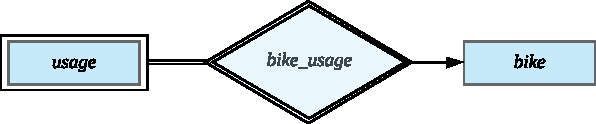
\includegraphics{figures/usage.pdf}
  \caption{\textit{usage}}
  \label{fig:usage}
\end{figure}

显然,实体集\textit{trace}应完全参与该关系集。
\paragraph{\textit{user\_feedback}}
如图\ref{fig:feedback}所示,关系集\textit{user\_feedback}将实体集\textit{bike,user}联系在一起。

该关系集表达的是“用户反馈单车故障”这一过程中,“单车”与“用户”之间的关系。

\begin{figure}[htbp]
  \centering
  \includegraphics{figures/user_feedback.pdf}
  \caption{\textit{user\_feedback}}
  \label{fig:feedback}
\end{figure}

用户反馈中的信息十分重要,这里我将反馈的时间\textit{time}和反馈的损坏器件\textit{component}作为该关系集的描述属性。因为
一次反馈可以反馈多处损坏,所以\textit{component}为多值属性。